\section{Moment-Generating Function}
\label{sec:mgf}\label{sec:3.4}

The moment-generating function (MGF) is a tool that encodes all the information of a probability distribution into a single function.

\begin{definicion}[Moment-Generating Function]
Let $X$ be a random variable. Its \emph{moment-generating function} (MGF) is
\begin{align}
 \label{eq:2.8.11}
 M_X(t) = E\!\left[e^{tX}\right].
\end{align}
If $X$ is discrete with probability function $f$,
\begin{align}
 M_X(t) = \sum_x e^{tx} f(x).
\end{align}
If $X$ is continuous with density function $f$,
\begin{align}
 M_X(t) = \int_{-\infty}^{\infty} e^{tx} f(x)\,dx.
\end{align}
\end{definicion}

The MGF exists if the integral or sum converges in an open interval around $t=0$.

\subsection{Moments from the MGF}

\begin{teorema}[Derivatives and Moments]
If $M_X(t)$ is the MGF of $X$, then for all $n \in \mathbb{N}$,
\begin{align}
 \label{eq:2.8.12}
 E\!\left[X^n\right] = M_X^{(n)}(0) = \left.\frac{d^n M_X(t)}{dt^n}\right|_{t=0}.
\end{align}
\end{teorema}

\begin{proof}
Interchanging differentiation and expectation (under regularity conditions):
\begin{align}
 M_X^{(n)}(t) = \frac{d^n}{dt^n}E[e^{tX}] = E\!\left[\frac{d^n}{dt^n}e^{tX}\right]
 = E\!\left[X^n e^{tX}\right].
\end{align}
Evaluating at $t=0$ yields $M_X^{(n)}(0) = E[X^n]$.
\end{proof}

\subsection{Uniqueness and Additive Property}

\begin{teorema}[Uniqueness]
If two random variables have the same MGF on an open interval around $t=0$, then they have the same probability distribution.
\end{teorema}

\begin{teorema}[Additive Property]
If $X$ and $Y$ are independent random variables, then
\begin{align}
 \label{eq:2.8.13}
 M_{X+Y}(t) = M_X(t)\,M_Y(t).
\end{align}
\end{teorema}

\begin{proof}
By independence,
\begin{align}
 M_{X+Y}(t) = E[e^{t(X+Y)}] = E[e^{tX}e^{tY}] = E[e^{tX}]\,E[e^{tY}] = M_X(t)\,M_Y(t).
\end{align}
\end{proof}

\subsection{Examples of MGFs}

\begin{ejemplo}
 \label{exmp:2.8.4}
Find the MGF of the Bernoulli distribution with parameter $p$.
\end{ejemplo}

\begin{solucion}
If $X \sim \text{Bernoulli}(p)$, then $P(X=1) = p$ and $P(X=0) = 1-p$.
\begin{align}
 M_X(t) = E[e^{tX}] = e^{0 \cdot t}(1-p) + e^{1 \cdot t}p
 = (1-p) + p\,e^t.
\end{align}

We check the moments:
\begin{align}
 M_X'(t) = p\,e^t &\implies E[X] = M_X'(0) = p. \\
 M_X''(t) = p\,e^t &\implies E[X^2] = M_X''(0) = p. \\
 \text{Var}(X) = E[X^2] - (E[X])^2 &= p - p^2 = p(1-p).
\end{align}
\end{solucion}

\begin{ejemplo}
 \label{exmp:2.8.5}
Find the MGF of the normal distribution $N(\mu, \sigma^2)$.
\end{ejemplo}

\begin{solucion}
Without loss of generality, consider $Z \sim N(0,1)$. Then
\begin{align}
 M_Z(t) &= \int_{-\infty}^{\infty} e^{tz}\,\frac{1}{\sqrt{2\pi}}e^{-z^2/2}\,dz \\
 &= \int_{-\infty}^{\infty} \frac{1}{\sqrt{2\pi}}\,\exp\!\left(tz - \frac{z^2}{2}\right)dz.
\end{align}

We complete the square: $tz - z^2/2 = -\frac{1}{2}(z - t)^2 + \frac{t^2}{2}$. Therefore,
\begin{align}
 M_Z(t) = e^{t^2/2}\int_{-\infty}^{\infty} \frac{1}{\sqrt{2\pi}}e^{-(z-t)^2/2}\,dz = e^{t^2/2}.
\end{align}
(the integral equals $1$ because it is the integral of the $N(t, 1)$ density function).

For $X \sim N(\mu,\sigma^2)$ we write $X = \mu + \sigma Z$, hence
\begin{align}
 \label{eq:2.8.14}
 M_X(t) = E[e^{tX}] = e^{t\mu}E[e^{t\sigma Z}] = e^{t\mu}\,e^{(\sigma t)^2/2}
 = \exp\!\left(\mu t + \frac{\sigma^2 t^2}{2}\right).
\end{align}
\end{solucion}

\begin{ejemplo}
 \label{exmp:2.8.6}
Find the MGF of the exponential distribution with parameter $\lambda$.
\end{ejemplo}

\begin{solucion}
If $X \sim \text{Exp}(\lambda)$, then
\begin{align}
 M_X(t) = \int_0^\infty e^{tx}\,\lambda e^{-\lambda x}\,dx
 = \lambda\int_0^\infty e^{-(\lambda - t)x}\,dx = \frac{\lambda}{\lambda - t},
\end{align}
for $t < \lambda$. Therefore,
\begin{align}
 \label{eq:2.8.15}
 M_X(t) = \frac{\lambda}{\lambda - t} = \left(1 - \frac{t}{\lambda}\right)^{-1},
 \qquad t < \lambda.
\end{align}

The moments are obtained by differentiation:
\begin{align}
 E[X^n] = \frac{n!}{\lambda^n}.
\end{align}
In particular, $E[X] = 1/\lambda$ and $\text{Var}(X) = 1/\lambda^2$.
\end{solucion}

\lstinputlisting[language=Python]{../code/distribuciones-continuas-avanzadas/fgmDistribuciones.py}

\begin{figure}
 \centering
 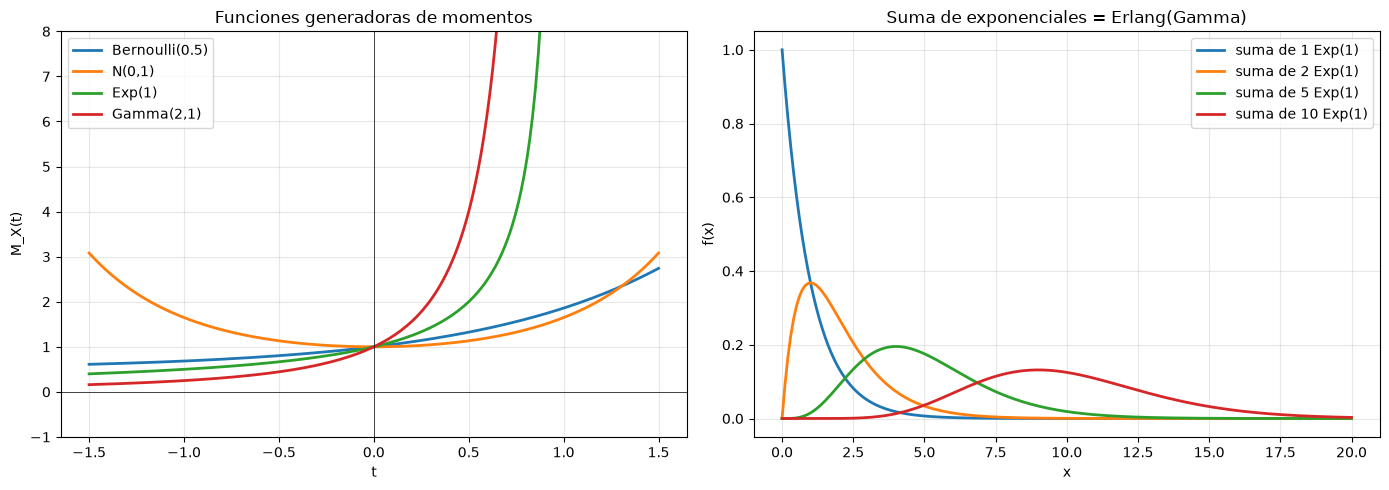
\includegraphics[height=7cm,keepaspectratio=true]{./pe/fgmDistribuciones.png}
 % fgmDistribuciones.png: 0x0 pixel, 300dpi, 0.00x0.00 cm, bb=
 \caption{Moment-generating functions and sum of independent gamma variables.}
 \label{fig:2.8.4}
\end{figure}

{Summary Table of MGFs}
\begin{center}
\begin{tabular}{|l|l|}
\hline
\textbf{Distribution} & \textbf{MGF $M_X(t)$} \\
\hline
Bernoulli$(p)$ & $(1-p) + p\,e^t$ \\
Binomial$(n,p)$ & $(1 - p + p\,e^t)^n$ \\
Poisson$(\lambda)$ & $\exp(\lambda(e^t - 1))$ \\
Geometric$(p)$ & $\dfrac{p\,e^t}{1 - (1-p)e^t}$ \\
Exponential$(\lambda)$ & $\dfrac{\lambda}{\lambda - t}$ \\
Normal$(\mu, \sigma^2)$ & $\exp\!\left(\mu t + \dfrac{\sigma^2 t^2}{2}\right)$ \\
Gamma$(\alpha, \beta)$ & $(1 - \beta t)^{-\alpha}$ \\
Chi-square$_\nu$ & $(1 - 2t)^{-\nu/2}$ \\
\hline
\end{tabular}
\end{center}

\begin{observacion}
The additive property for independent random variables is easily applied: if $X_1, \dots, X_n$ are i.i.d. Bernoulli$(p)$, then $\sum X_i \sim \text{Binomial}(n,p)$ and
\begin{align}
 M_{\sum X_i}(t) = \prod_{i=1}^n M_{X_i}(t) = (1 - p + p\,e^t)^n,
\end{align}
which coincides with the MGF of the binomial distribution.
\end{observacion}
